\documentclass{article}

\usepackage{amsmath}
\usepackage{amssymb}
\usepackage{hyperref}
\usepackage{url}
\usepackage{graphicx}
\usepackage{geometry}
\usepackage[italian]{babel}
\usepackage{enumitem}
\usepackage{parskip}
\usepackage{chemfig}
\usepackage{pdfpages}
\usepackage[table]{xcolor}
\usepackage{tikz}
\usepackage{fancybox}
\usepackage{makecell}
\usepackage{soul}
\usepackage{sankey}
\usepackage{caption}
\usepackage{lipsum}
\usepackage{pgfplots}
\pgfplotsset{compat=1.17}
\usepackage{ulem}
\usepackage{wrapfig}
\usepackage{subcaption}
\usepackage{svg}
\usepackage{array}
\usepackage[utf8]{inputenc}
\usepackage{multirow}


\usetikzlibrary{shapes.geometric, arrows}
\usetikzlibrary{decorations.pathreplacing}
\usetikzlibrary{arrows.meta}

\geometry{
    a4paper,
    total={170mm, 257mm},
    left=20mm,
    top=20mm
}

\hypersetup{
    colorlinks=true,
    linkcolor=black,
    urlcolor=blue,
    pdftitle={Biologia}
}

\definecolor{darkgreen}{rgb}{0.0, 0.7, 0.0}

% === COMMANDS ===
\newcommand{\figbox}[1]{
    \begin{figure*}[ht!]
        \begin{center}
            \fbox{#1}
        \end{center}
    \end{figure*}
}

\newcommand*\circled[1]{\tikz[baseline=(char.base)]{
            \node[shape=circle,draw,inner sep=1.1pt] (char) {#1};}
}
\newcommand\angstrom{\mbox{\normalfont\AA}}
\newcommand\namebond[4][5pt]{\chemmove{\path(#2)--(#3)node[midway,sloped,yshift=#1]{#4};}}
\newcommand\arcbetweennodes[3]{
    \pgfmathanglebetweenpoints{\pgfpointanchor{#1}{center}}{\pgfpointanchor{#2}{center}}
    \let#3\pgfmathresult
}
\newcommand\arclabel[8][stealth-stealth,shorten <=1pt,shorten >=1pt]{
    \chemmove{
        \arcbetweennodes{#4}{#3}\anglestart \arcbetweennodes{#4}{#5}\angleend
        \draw[#1]([shift=(\anglestart:#2)]#4)arc(\anglestart:\angleend:#2);
        \pgfmathparse{(\anglestart+\angleend)/2}\let\anglestart\pgfmathresult
        \node[shift=(\anglestart:#2+1pt)#4,anchor=\anglestart+180,rotate=\anglestart#7,
        inner sep=0pt,outer sep=#8]at(#4){#6};
    }
}

\newcommand\hr{\vspace{0.1cm}\par\vspace{-.5\ht\strutbox}\noindent\hrulefill\par\vspace{0.1cm}}

% Fill the remaining space of a wrapfigure
\newcommand{\wrapfill}{
    \par
    \ifnum \value{WF@wrappedlines} > 0
        \addtocounter{WF@wrappedlines}{-1}%
        \null\vspace{
            \arabic{WF@wrappedlines}
            \baselineskip
        }
        \WFclear
    \fi
    \phantom{}
}

\newcommand{\cfig}[2]{
    \phantom{}
    \begin{figure*}[ht!]
        \begin{center}
            \includegraphics[width=#1\textwidth]{#2}
        \end{center}
    \end{figure*}
}

\newcommand{\chemscheme}[1]{
    \\
    \phantom{}
    \figbox{
        \schemestart
        #1
        \schemestop
    }
}

% === TEXT ===
\title{\textbf{Biologia \\ Passerella 2023-24}}
\author{Matteo Frongillo}

\begin{document}

\maketitle
\tableofcontents
\pagebreak

\part{Biologia umana}
\section{Sistema vivente}
La classificazione di sistema vivente è suddivisa in due macrocategorie:
\begin{itemize}
    \item \textbf{Visione meccanicistica}: Un sistema vivente è riconosciuto come tale
        se possiede questi elementi:
        \begin{itemize}
            \item Basi cellulari;
            \item Ha una forma e una funzione;
            \item Codice genetico (XNA);
            \item Scambio di materia e di energia;
            \item Ciclo vitale e riproduzione;
            \item Reazione agli stimoli;
            \item Omeostasi;
            \item Evoluzione e varietà.
        \end{itemize}
    \item \textbf{Visione sistemica}: Un sistema vivente è riconosciuto come tale
        se possiede questi elementi:
        \begin{itemize}
            \item \textbf{Sistema autoconfinato:} autoproduce ciclicamente i propri componenti;
            \item \textbf{Sistema autopoietico:} mantiene la propria organizzazione e identità
                attraverso la rigenerazione dei propri componenti;
            \item \textbf{Struttura cognitiva:} adatta i propri processi interni per mantenere
                l'equilibrio con l'esterno;
            \item \textbf{Struttura dissipativa:} scambiano materia con l'ambiente, assorbendo
                nutrienti ed espellendo rifiuti.
        \end{itemize}
\end{itemize}

\newpage
\section{Gli organismi}
\subsection{Le caratteristiche}
Un organismo è un essere vivente che possiede le seguenti caratteristiche:

\subsubsection{Nutrizione (dissipazione)}
Esistono due tipi di nutrizioni per gli organismi:
\begin{enumerate}
    \item Organismi autotrofi: assimilano il cibo da soli e fanno la fotosintesi o chemiosintesi:
        \begin{itemize}
            \item \textbf{Fotosintesi:} ha bisogno di \underline{energia solare} e una
                pigmentazione verde.\\
                La sua formula chimica è:

                \begin{center}
                    \schemestart
                    CO$_2$ + H$_2$O \arrow{->[energia][solare]} C$_6$H$_{12}$O$_6$ (glucosio) + O$_2$
                    \schemestop ;
                \end{center} \phantom{}

            \item \textbf{Chemiosintesi:} gli organismi ottengono energia dall'ossidazione di
                composti inorganici.\\
                La formula chimica è:

                \begin{center}
                    \schemestart
                    CO$_2$ + H$_2$O + 3H$_2$S \arrow{->} C$_6$H$_{12}$O$_6$ + H$_2$SO$_4$
                    \schemestop ;
                \end{center} \phantom{}
                
        \end{itemize}
    \item Organismi eterotrofi: assimilano il cibo da materia organica viva o morta.
\end{enumerate}

\paragraph{La nutrizione degli esseri viventi:}
\begin{itemize}
    \item Animali: sono eterotrofi e si nutrono di cibo, dunque fatta di materia organica;
    \item Piante: sono autotrofe e si nutrono di CO$_2$, dunque materia inorganica;
    \item Funghi: sono eterotrofi e si nutrono di materia organica.
\end{itemize}

\subsubsection{Respirazione (dissipazione)}
Esistono due tipi di respirazione:
\begin{enumerate}
    \item Respirazione cellulare: 
        \begin{center}
            \begin{tikzpicture}
                \begin{sankeydiagram}[start style=arrow,end style=arrow]
                    \sankeynodestart{quantity=15, name=node1, at={0,0}}
                    \node[left=0.5cm, above, rotate=90] (label1) {C$_6$H$_{12}$O$_6$ + O$_2$};
                    
                    \sankeyadvance{node1}{2cm}
                    \sankeyfork{node1}{5/node2, 10/node3}
            
                    \sankeyturn{node2}{90}
                    \sankeyadvance{node2}{.2cm}
                    \sankeyend{node2}
                    \node[above=2.1cm, right=2cm] (label2) {Energia};
            
                    \sankeyturn{node3}{0}
                    \sankeyadvance{node3}{1cm}
                    \sankeyend{node3}
                    \node[above=-0.26cm, right=3.5cm] (label2) {CO$_2$ + H$_2$O};
                \end{sankeydiagram}.
            \end{tikzpicture}
        \end{center}
    \item Fermentazione:
        \begin{itemize}
            \item Alcolica (lieviti): è un processo anaerobico in cui i lieviti e alcuni batteri
                convertono il glucosio in etanolo e anidride carbonica, con formula chimica:

                \begin{center}
                    \schemestart
                    C$_6$H$_{12}$O$_6$ \arrow{->} 2C$_3$H$_6$O$_3$
                    \schemestop

                    \schemestart
                    2C$_3$H$_6$O$_3$ \arrow{->[lieviti]} 2C$_2$H$_5$OH + 2CO$_2$
                    \schemestop;
                \end{center}
                
                \phantom{}
            \item Lattica (batteri): è un processo anaerobico in cui il glucosio viene
                convertito in acido lattico. Questo avviene nei muscoli durante l'esercizio
                fisico intenso e in alcuni batteri e ha come formula chimica:

                \begin{center}
                    \schemestart
                    C$_6$H$_{12}$O$_6$ \arrow{->} 2C$_3$H$_6$O$_3$
                    \schemestop.
                \end{center}
        \end{itemize}
\end{enumerate}

\newpage
\subsubsection{Riproduzione e ciclo vitale (autopoiesi)}
Ha una struttura ciclica vitale:\\
Nascita\ \textrightarrow\ Crescita\ \textrightarrow\ Riproduzione\ \textrightarrow\ Morte

\subsubsection{Evoluzione (cognizione)}
Un organismo si adatta all'ambiente circostante per migliorare la proria vita.

\subsubsection{Sensibità (cognizione)}
Risponde all'ambiente per l'evoluzione ed altri fattori

\subsubsection{Stabilità}
Mantiene stabili le sue condizioni interne.

\subsection{Classificazione}
\subsubsection{Biotico}
\begin{itemize}
    \item \textbf{Organismo:} essere vivente;
    \item \textbf{Detrito:} ex essere vivente, morto.
\end{itemize}

\subsubsection{Abiotico}
\textbf{Non vivente:} senza le caratteristiche di un essere vivente.

\subsection{Concetto di fattore}
\begin{itemize}
    \item Componente: materia, qualcosa di concreto e tangibile;
    \item Fattore: deriva dalla presenza di componenti, produce un determinato effetto o
        risultato e \underline{si può misurare}.
        Ad esempio:
        \begin{itemize}
            \item Decomposizione (biotico);
            \item Predazione, catena alimentare (biotico);
            \item Vento (abiotico);
            \item Luce solare (abiotico).
        \end{itemize}
\end{itemize}

\newpage
\section{Biochimica}
Le biomolecole sono le molecole dei processi biologici degli esseri viventi.
Quelle che si trovano nella biologia umana sono principalmente:
\begin{center}
    \[
        \underbrace{{\begin{array}{c}
            \text{C}\qquad
            \text{O}\qquad
            \text{H}\qquad 
        \end{array}}}_{\text{in tutte le molecole}}\quad
        \begin{array}{c}
            \text{N}\qquad
            \text{S}\qquad
            \text{P}\qquad
        \end{array}
    \]
\end{center}

\subsection{Classificazione delle biomolecole}
\begin{itemize}
    \item Lipidi (grassi);
    \item Acidi nucleici (DNA, xRNA);
    \item Carboidrati (zuccheri);
    \item Proteine.
\end{itemize}

\subsection{Sintesi delle macromolecole}
\begin{itemize}
    \item Monomeri: componenti singole;
    \item Polimeri: composizione di 2 o più monomeri.
\end{itemize}

\subsection{Reazione di disidratazione (condensazione)}
La condensazione tra due polimeri serve ad unirli assieme, in modo da formare una catena singola.
Questo procedimento ha lo scopo di minimizzare lo spazio occupato dai polimeri. 
\begin{figure*}[ht!]
    \vspace*{0.5cm}
    \begin{center}
        \begin{tikzpicture}
            % First molecule (top left)
            \draw (0, 1) node {H};
            \draw (1, 1) circle (0.3);
            \draw (2, 1) circle (0.3);
            \draw (3, 1) circle (0.3);
            \draw (4, 1) node {OH};
            \draw (0.3, 1) -- (0.7, 1);
            \draw (1.3, 1) -- (1.7, 1);
            \draw (2.3, 1) -- (2.7, 1);
            \draw (3.3, 1) -- (3.7, 1);
            
            % Second molecule (top right)
            \draw (6, 1) node {H};
            \draw (7, 1) circle (0.3);
            \draw (8, 1) node {OH};
            \draw (6.3, 1) -- (6.7, 1);
            \draw (7.3, 1) -- (7.7, 1);
            
            % Arrow pointing down
            \draw[-{Latex[scale=2]}] (5, 1) -- (5, -1.5);
            
            % Water molecule
            \draw[-{Latex[scale=2]}] (5, 0) to[out=270,in=180] (5.5, -0.5) to[out=180,in=180] (6.1, -0.5);
            \draw (6.5, -0.5) circle (0.4) node {H$_2$O};
            
            % Resulting molecule (bottom)
            \draw (1.5, -2) node {H};
            \draw (2.5, -2) circle (0.3);
            \draw (3.5, -2) circle (0.3);
            \draw (4.5, -2) circle (0.3);
            \draw (5.5, -2) circle (0.3);
            \draw (6.5, -2) node {OH};
            \draw (1.8, -2) -- (2.2, -2);
            \draw (2.8, -2) -- (3.2, -2);
            \draw (3.8, -2) -- (4.2, -2);
            \draw (4.8, -2) -- (5.2, -2);
            \draw (5.8, -2) -- (6.2, -2);
        \end{tikzpicture}
    \end{center}
\end{figure*}

\subsection{Reazione di idratazione (idrolisi)}
L'idrolisi tra due polimeri serve a dividere una parte di una catena esistente, in modo da
formare due catene distinte.
Questo procedimento ha come scopo la divisione di un monomero pronto per essere usato da una
catena di polimeri. 
\begin{figure*}[ht!]
    \vspace*{0.5cm}
    \begin{center}
        \begin{tikzpicture}
            % Resulting molecule (top)
            \draw (1.5, 2) node {H};
            \draw (2.5, 2) circle (0.3);
            \draw (3.5, 2) circle (0.3);
            \draw (4.5, 2) circle (0.3);
            \draw (5.5, 2) circle (0.3);
            \draw (6.5, 2) node {OH};
            \draw (1.8, 2) -- (2.2, 2);
            \draw (2.8, 2) -- (3.2, 2);
            \draw (3.8, 2) -- (4.2, 2);
            \draw (4.8, 2) -- (5.2, 2);
            \draw (5.8, 2) -- (6.2, 2);
            
            % Arrow pointing down
            \draw[-{Latex[scale=2]}] (5, 1.5) -- (5, -1);
            
            % Water molecule
            \draw[-{Latex[scale=2]}] (6.1, 0.5) to[out=180,in=0] (5.85, 0.5) to[out=180,in=60] (5.05, -0.25);
            \draw (6.5, 0.5) circle (0.4) node {H$_2$O};
        
            % First molecule (bottom left)
            \draw (0, -1) node {H};
            \draw (1, -1) circle (0.3);
            \draw (2, -1) circle (0.3);
            \draw (3, -1) circle (0.3);
            \draw (4, -1) node {OH};
            \draw (0.3, -1) -- (0.7, -1);
            \draw (1.3, -1) -- (1.7, -1);
            \draw (2.3, -1) -- (2.7, -1);
            \draw (3.3, -1) -- (3.7, -1);
            
            % Second molecule (bottom right)
            \draw (6, -1) node {H};
            \draw (7, -1) circle (0.3);
            \draw (8, -1) node {OH};
            \draw (6.3, -1) -- (6.7, -1);
            \draw (7.3, -1) -- (7.7, -1);
        \end{tikzpicture}
    \end{center}
\end{figure*}

\newpage
\subsection{Carboidrati}
I carboidrati sono (quasi tutti) composti dagli elementi C, O e H (composti idratati del
carbonio). Questi composti hanno formula (CH$_2$O)$_n$.

Tutti i carboidrati sono \textbf{isomeri}, ossia hanno tutti la stessa formula chimica ma con
gli elementi chimici disposti in maniera fisicamente differente.

\begin{figure*}[ht!]
    \vspace*{0.5cm}
    \begin{tikzpicture}[scale=0.5]
    
        % MONOSACCARIDI
        \coordinate (A) at (0, 0);
        \coordinate (B) at (1, 1.5);
        \coordinate (C) at (4, 1.5);
        \coordinate (D) at (5, 0);
        \coordinate (E) at (4, -1.5);
        \coordinate (F) at (1, -1.5);
    
        \draw (A) -- (B) -- (C) -- (D) -- (E) -- (F) -- cycle;
    
        \node at (12.5,0) {Monosaccaridi (glucosio, fruttosio, galattosio)};
    
        % DISACCARIDI
        \coordinate (A) at (0, -5);
        \coordinate (B) at (1, -3.5);
        \coordinate (C) at (4, -3.5);
        \coordinate (D) at (5, -5);
        \coordinate (E) at (4, -6.5);
        \coordinate (F) at (1, -6.5);
    
        \draw (A) -- (B) -- (C) -- (D) -- (E) -- (F) -- cycle;
    
        \coordinate (A1) at (6.5, -5);
        \coordinate (B1) at (7.5, -3.5);
        \coordinate (C1) at (10.5, -3.5);
        \coordinate (D1) at (11.5, -5);
        \coordinate (E1) at (10.5, -6.5);
        \coordinate (F1) at (7.5, -6.5);
    
        \draw (A1) -- (B1) -- (C1) -- (D1) -- (E1) -- (F1) -- cycle;
    
        \draw[thick] (5, -5) -- (6.5, -5);
    
        \node at (18.5,-5) {Disaccaridi (saccarosio, lattosio, maltosio)};
    
        % POLISACCARIDI
        \coordinate (A) at (0, -10);
        \coordinate (B) at (1, -8.5);
        \coordinate (C) at (4, -8.5);
        \coordinate (D) at (5, -10);
        \coordinate (E) at (4, -11.5);
        \coordinate (F) at (1, -11.5);
    
        \draw (A) -- (B) -- (C) -- (D) -- (E) -- (F) -- cycle;
    
        \coordinate (A1) at (6.5, -10);
        \coordinate (B1) at (7.5, -8.5);
        \coordinate (C1) at (10.5, -8.5);
        \coordinate (D1) at (11.5, -10);
        \coordinate (E1) at (10.5, -11.5);
        \coordinate (F1) at (7.5, -11.5);
    
        \draw (A1) -- (B1) -- (C1) -- (D1) -- (E1) -- (F1) -- cycle;
    
        \draw[thick] (5, -10) -- (6.5, -10);
    
        \coordinate (A2) at (13, -10);
        \coordinate (B2) at (14, -8.5);
        \coordinate (C2) at (17, -8.5);
        \coordinate (D2) at (18, -10);
        \coordinate (E2) at (17, -11.5);
        \coordinate (F2) at (14, -11.5);
    
        \draw (A2) -- (B2) -- (C2) -- (D2) -- (E2) -- (F2) -- cycle;
    
        \draw[thick] (11.5, -10) -- (13, -10);
    
        \node at (25,-10) {Polisaccaridi (amido, cellulosa, glicogeno)};
    \end{tikzpicture}
\end{figure*}

\subsubsection{Monosaccaridi}
I monosaccaridi hanno formula chimica C$_6$H$_{12}$O$_6$:\\
\phantom{}

\begin{minipage}{0.2\textwidth}
    \centering
    \chemfig[cram width=2pt]{
        HO-[2,0.5,2]?<[7,0.7](-[2,0.5]OH)-[,,,,line width=2pt](-[6,0.5]OH)>[1,0.7](-[6,0.5]OH)
        -[3,0.7]O-[4]?(-[2,0.3]-[3,0.5]CH_2OH)
    } \phantom{}\\
    \hspace*{0.5cm} Glucosio
\end{minipage}
\hspace{3cm}
\begin{minipage}{0.2\textwidth}
    \centering
    \chemfig[cram width=2pt]{
        HO-[2,-0.5,2]?<[7,0.7](-[2,0.5]OH)-[,,,,line width=2pt](-[6,0.5]OH)>[1,0.7](-[6,0.5]OH)
        -[3,0.7]O-[4]?(-[2,0.3]-[3,0.5]CH_2OH)
        } \phantom{}\\
        \hspace*{0.5cm} Galattosio
\end{minipage}
\hspace{3cm}
\begin{minipage}{0.2\textwidth}
    \centering
    \chemfig[cram width=2pt]{
        (?[a](-[2]CH_2OH)
        <[7,0.7](-[6,0.5]OH)-[,,,,line width=2pt](-[2,0.5,,2]HO)>[1,0.7](-[6,0.5]CH_2OH)
        -[:150,1.15]O?[a])
        } \phantom{}\\
        \hspace*{-0.5cm} Fruttosio
\end{minipage}

\subsubsection{Disaccaridi}
I disaccaridi sono coppie di monosaccaridi con formula chimica C$_{12}$H$_{22}$O$_{11}$:
\begin{itemize}
    \item Glucosio + Galattosio: \underline{Lattosio};
    \item Glucosio + Glucosio: \underline{Maltosio};
    \item Glucosio + Fruttosio: \underline{Saccarosio}.
\end{itemize}

\subsubsection{Polisaccaridi}
I polisaccaridi sono catene di monosaccaridi:
\begin{itemize}
    \item Amido: si trova nelle piante e serve a ricavare il glucosio tramite il processo di
        amilasi. La struttura è elicoidale e serve per occupare meno spazio nelle cellule.
        \begin{figure*}[ht!]
            \centering
            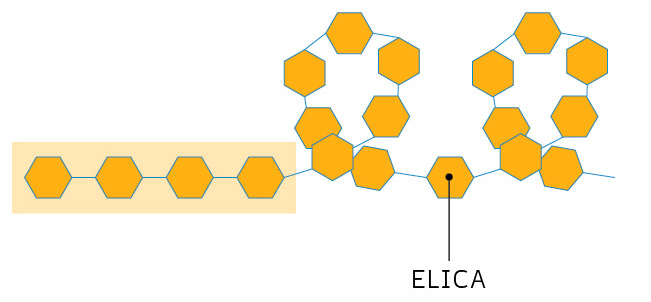
\includegraphics[width=0.4\textwidth]{media/amido.png}
        \end{figure*}
    \newpage
    \item \textbf{Glicogeno}: si trova negli esseri viventi ed è una catena elicoidale di
        monosaccaridi, anch'esso a scopo di ricavare il glucosio tramite il processo di amilasi.
        \begin{figure*}[ht!]
            \centering
            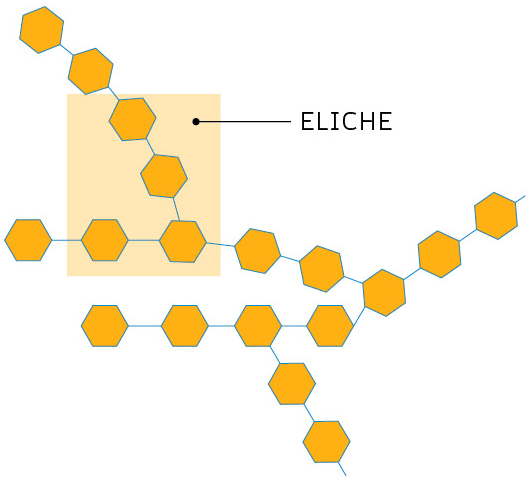
\includegraphics[width=0.4\textwidth]{media/glicogeno.png}
        \end{figure*}

    \item \textbf{Cellulosa:} la sua funzione principale è essere una \underline{struttura}.
        Viene utilizzata come riserva per la produzione di energia solo in caso estremi.
        \begin{figure*}[ht!]
            \centering
            \includegraphics*[width=0.4\textwidth]{media/cellulosa.png}
        \end{figure*}
\end{itemize}

\subsubsection{Enzimi}
\paragraph{$\alpha$-amilasi} \phantom{}

L'enzima $\alpha$-amilasi catalizza la degradazione dell'amido in zuccheri semplici come il
maltosio e il glucosio. Il processo di amilasi inizia nella bocca, grazie all'amilasi salivare,
e continua nell'intestino tenue con l'amilasi pancreatica.

\paragraph{Isomerasi} \phantom{}

L'enzima isomerasi catalizza la conversione di una molecola in uno dei suoi isomeri. Il processo
di isomerizzazione permette il cambiamento della struttura molecolare senza alterare il numero
di atomi (es. da monomeri di glucosio a monomeri di fruttosio).

\newpage
\subsection{Acidi nucleici - nucleotidi}
Gli acidi nucleici sono composti da un gruppo fosfato, uno zucchero e una base azotata.

\subsubsection{Gruppo fosfato}
Il gruppo fosfato è un gruppo funzionale presente negli acidi nucleici che lega insieme i
nucleotidi, formando lo scheletro esterno della struttura a doppia elica del DNA o dell'xRNA.
\figbox{
    \chemfig{
        O=P(-[:90]O^{-})(-[:-90]O^{-})-O-R
    }
}

\subsubsection{Carboidrati}
Il gruppo carboidrato è costituito da una molecola di \underline{ribosio} nell'RNA o da una
molecola di \underline{deossiribosio} nel DNA. Esempio di un acido nucleico DNA (deossiribosio):
\figbox{\hspace*{1.6cm}
    \chemfig[cram width=2pt]{
        (?[a](-[2]CH_2-[:180]\text{\hspace{-1.75cm} Gruppo fosfato})<[7,0.7](-[6,0.5]OH-[6,0.75]
        {\color{red}{R}})-[,,,,line width=2pt](-[2,-0.5]H)>[1,0.7](-[6,-0.5]\text{\hspace*{1.6cm}
        Base azotata})-[:150,1.15]O?[a])
    }
}

La {\color{red}R} rappresenta una delle quattro possibili basi azotate che possono legarsi
al ribosio (A, T, C, G).

\subsubsection{Base azotata}
La base azotata è una molecola organica che serve a codificare le informazioni genetiche,
con sequenze specifiche di base (Adenina, Timina, Citosina, Guanina e Uracile) che determinano
le istruzioni per la sintesi delle proteine e il funzionamento delle cellule.
Esempio con la base azotata uracile:
\figbox{
    \chemfig{
        [:60]R-[:90]N*6(-(=[:-30]O)-N-(=[:90]O)-=-)
    }
}

\subsubsection{Polinucleotidi}
I polinucleotidi sono una coppia di nucleotidi elicoidali che formano una struttura a doppia
elica:
\begin{figure*}[ht!]
    \begin{center}
        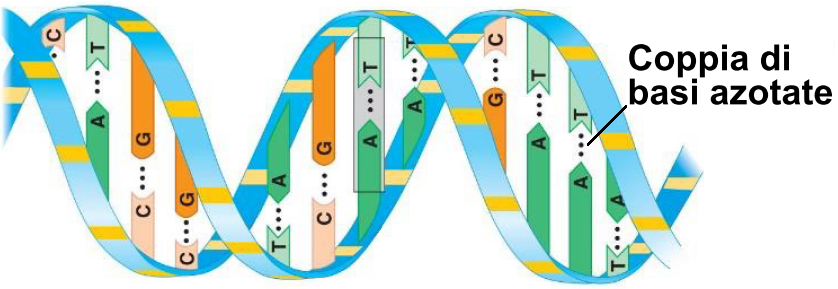
\includegraphics[width=0.4\textwidth]{media/doppia_elica.png}
    \end{center}
\end{figure*}

\subsection{Proteine - amminoacidi}
La proteina è una catena di amminoacidi (20 tipi diversi) e sono caratterizzate da un gruppo
amminico, un gruppo carbossilico e una struttura resto (R).
\figbox{
    \chemfig{
        N(-[:135]H)(-[:-135]H)-\circled{C}(-[:90]H)(-[:-90]R)-C(=[:45]O)(-[:-45]OH)
    }
}

\subsubsection{Gruppo amminico}
Il gruppo amminico (-NH$_2$) serve a formare legami peptidici con il gruppo carbossilico di un
altro amminoacido, consentendo la costruzione della catena polipeptidica.

\subsubsection{Gruppo carbossilico}
Il gruppo carbossilico (-COOH) serve a formare legami peptidici con il gruppo amminico di un
altro amminoacido, consentendo la costruzione della catena polipeptidica.

\subsubsection{Gruppo resto}
Il gruppo resto (R) di un amminoacido determina le proprietà chimiche e la funzione
dell'amminoacido, variando tra 20 diverse catene laterali che conferiscono specificità e
diversità alle proteine.

\subsubsection{Struttura}
\begin{center}
    \begin{tikzpicture}
        % Struttura primaria (lineare)
        \draw[thick] (0,2.25) -- (10,2.25);
        \foreach \x in {1,2,...,9} {
            \draw[fill=yellow] (\x,2.25) circle (0.2);
        }
        
        \node at (5,1.7) {Struttura primaria - Lineare};
        
        % Struttura secondaria (elicoidale)
        \draw[thick,domain=0:10,smooth,variable=\x] plot ({\x},{sin(2*\x r)});
        \foreach \x in {0.785,1.57,...,10.205} {
            \draw[fill=yellow] (\x,{sin(2*\x r)}) circle (0.2);
        }
        
        \node at (5,-1.75) {Struttura secondaria - Elicoide};

        \node at (2.5,-4.75) {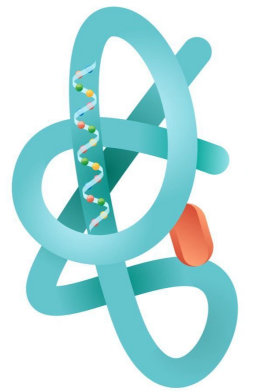
\includegraphics[width=.175\textwidth]{media/terziaria.png}};
        \node at (2.5,-7.5) {Struttura terziaria};
        \node at (7.5,-4.75) {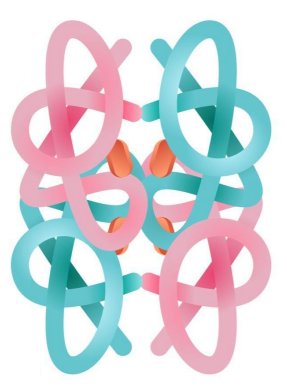
\includegraphics[width=.2\textwidth]{media/quaternaria.png}};
        \node at (7.5,-7.5) {Struttura quaternaria};
    \end{tikzpicture}
\end{center}

\begin{itemize}
    \item Primaria: è composta linearmente da amminoacidi;
    \item Secondaria: ha sempre una forma elicoidale e può essere arrotolata su sé stessa,
        senza però avere nessuna funzionalità specifica (catena polipeptidica);  
    \item Terziaria: ha una struttura elicoidale arrotolata su sé stessa e ha una funzione;
    \item Quaternaria: aggregazione di uno o più polipeptidi terziari.
\end{itemize}

\subsubsection{Le funzioni delle proteine}
\begin{itemize}
    \item \textbf{Strutturali} (cheratina, elastina, collagine, ...): servono alla rigenerazione
        delle strutture, ad esempio la rigenerazione delle unghie, dei capelli o della pelle;
    \item \textbf{Contrattili} (actina, miosina, ...): servono a garantire la contrazione dei
        muscoli;
    \item \textbf{Di riserva} (albumina, caseina, glutine, ...): servono come riserva
        nutrizionale per gli animali, ad esempio i nutrienti all'interno di un uovo per gli
        ovipari oppure il latte per i mammiferi;
    \item \textbf{Di difesa} (anticorpi, ...): servono per proteggere l'organismo dagli agenti
        patogeni;
    \item \textbf{Di trasporto} (emoglobina, ...): servono a trasportare una molecola
        all'interno del corpo, ad esempio la molecola di ossigeno O$_2$ nel sangue;
    \item \textbf{Regolatrici} (insulina, ...): servono a regolare la qualità di una molecola
        nel corpo, ad esempio la regolazione dei livelli di glucosio per ridurre la glicemia;
    \item \textbf{Enzimi} (amilasi, ...): sono proteine che permettono lo svolgimento di
        reazioni chimiche all'interno delle cellule, ad esempio la reazione di idrolisi.
\end{itemize}

\newpage
\subsection{Lipidi - acidi grassi e glicerolo}

\subsubsection{Monogliceridi}
Gli acidi grassi non polimerizzano, poiché la coda è idrofoba.
\begin{center}
    \chemfig{
        H-[:-90]C(-[:180]H)(-OH)-[:-90]C(-[:180]H)(-OH)-[:-90]C(-[:180]H)(-[:-90]H)-OH(
        -O(-[:-90]H)-C(=[:90]O)-C(-[:90]H)(-[:-90]H)-C(-[:90]H)(-[:-90]H)-C(-[:90]H)(-[:-90]H)
        -C(-[:90]H)(-[:-90]H)-C(-[:90]H)(-[:-90]H)-C(-[:90]H)(-[:-90]H)-C(-[:90]H)(-[:-90]H)-H)
    }

\end{center}
\hspace*{1.725cm}   
$\underbrace{{\begin{array}{c}
    \phantom{CIAOCIAOC}
\end{array}}}_{\text{\normalsize Testa {\color{red}{idrofila}}}}$
\hspace*{1.5cm}   
$\underbrace{{\begin{array}{c}
    \phantom{CIAOCIAOCIAOCIAOCIAOCIAOCIAOCIAOCIA}
\end{array}}}_{\text{\normalsize Coda {\color{red}{idrofoba}}}}$

\subsubsection{Trigliceridi}
I trigliceridi sono la principale forma di \underline{deposito energetico} nei lipidi per la
produzione di ATP, composti da una molecola di glicerolo legata a tre acidi grassi attraverso
legami esterei.
\begin{figure*}[ht!]
    \begin{center}
        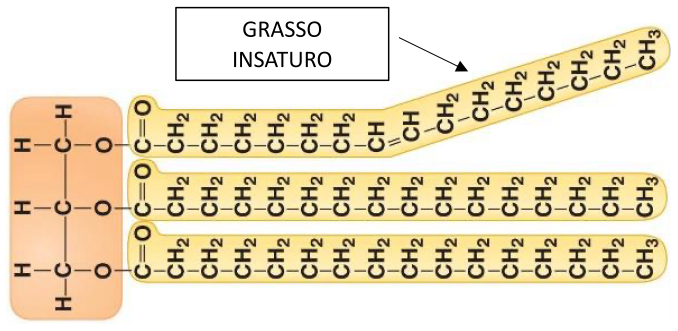
\includegraphics[width=0.55\textwidth]{media/trigliceridi.png}
    \end{center}
\end{figure*}

Nei trigliceridi, i grassi saturi hanno catene di acidi grassi senza doppi legami tra gli atomi
di carbonio, mentre i grassi insaturi contengono uno o più legami doppi, influenzando la
fluidità e il punto di fusione del grasso.

\subsubsection{Fosfolipidi}
I fosfolipidi sono formati da due acidi grassi e un gruppo fosfato legato a una molecola di
glicerolo, creando una struttura anfifilica con una testa idrofila e due code idrofobe.

\figbox{
    \chemfig{
        H_3N^{+}-[1]--[1]O-P(=[2]O)(-[1]O^{-})(-[-1]O(-[5]-[-1](<:O-[1](=[2])-[-1]-[1]-[-1]-[1]
        -[-1]-[1]-[2]CH_3)-[5]-[-1]O-[-1](=[6]O)-[1]-[-1]-[1]-[-1]-[1]-[-1]-[1]-[-1]-[6]CH_3))
    }
}

\subsubsection{Doppio strato di fosfolipidi}
Il doppio strato di fosfolipidi costituisce la struttura delle membrane cellulari, con le teste
idrofile orientate verso l'esterso e le code idrofobe rivolte verso l'interno, formando una
barriera semipermeabile.
\begin{figure*}[ht!]
    \begin{center}
        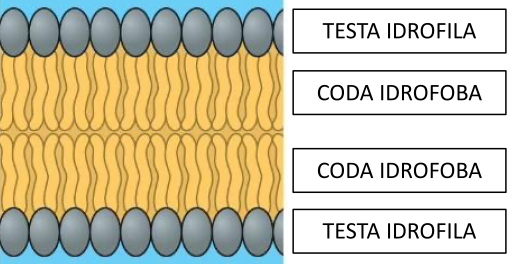
\includegraphics[width=0.5\textwidth]{media/membrana_cell.png}
    \end{center}
\end{figure*}

\subsubsection{Steroidi}
Gli steroidi sono molecole caratterizzate da un nucleo di \textbf{quattro anelli di carbonio}
e svolgono il ruolo di ormoni, componenti di membrane cellulari e regolatori del metabolismo.
Esempio del colesterolo:

\figbox{
    \chemfig{
        [:60]HO-[:30]*6(--(*6(=--(*6(-([:30]*5(---(-C(-[3]H_3C)-[1]-[-1]-[1]-[-1]-[1](-[:30]CH_3)
        -[:-60]CH_3)-(-[:90]CH_3)))----))--))-(-[:90]CH_3)---)
    }
}

\newpage
\section{Bioenergetica}
\subsection{Le membrane}
Ogni membrana del corpo di ogni cellula è formata spontaneamente da fosfolipidi immersi in
soluzioni acquose.

\subsubsection{Sistema aperto}
In un sistema aperto, la coda si allontana più possibile dall'acqua. Ad esempio, in un bicchiere
la testa del fosfolipide si troverà immersa, mentre la coda sarà rivolta verso l'esterno.

\subsubsection{Sistema chiuso}
In un sistema chiuso, i fosfolipidi formano un \textbf{compartimento}, così da esporre il meno
possibile la coda verso la soluzione:
\begin{figure*}[ht!]
    \begin{center}
        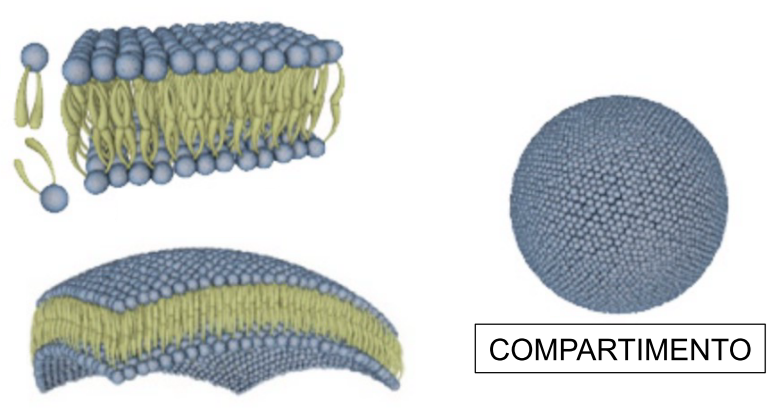
\includegraphics[width=.6\textwidth]{media/compartimento.png}
    \end{center}
\end{figure*}
Le vescicole sono compartimenti che trasportano al suo interno molecole molto grandi.

\subsection{Le proteine di membrana}
\subsubsection{Trasportatori}
Grazie all'ATP, il trasportatore investe energia per muovere una specifica molecola contro
gradiente, contrastando il suo movimento naturale.

\subsubsection{Canali}
È un canale di trasporto sempre aperto. Ogni canale trasporta una singola specifica molecola ed
è bidirezionale. Le sostanze si spostano per diffusione (gradiente), dunque si spostano da
dove c'è più concentrazione di una molecola verso una zona con meno concentrazione.

\subsubsection{Recettori}
I recettori sono proteine che si legano a specifiche molecole esterne alla cellula.
Questa interazione permette alla cellula di acquisire informazioni riguardanti le molecole
stesse, facilitando le risposte cellulari appropriate. Ad esempio, quando l'insulina si lega
al suo recettore, questo riconoscimento attiva una cascata di segnali che informano la cellula
di essere pronta ad assorbire il glucosio.

\newpage
\cfig{.9}{media/proteine_membrana.png}

\subsection{Trasporti}
\subsubsection{Diffusione semplice}
Il movimento delle molecole avviene attraverso la membrana senza l'uso di energia.

\subsubsection{Gradiente}
\begin{itemize}
    \item Elettrochimico: le molecole si spostano in base alle cariche elettriche parziali;
    \item Concentrazione: le molecole si spostano in base alla concentrazione.
\end{itemize}

\subsubsection{Trasporto attivo (contro gradiente)}
\begin{itemize}
    \item Primario: il trasporto avviene grazie all'energia derivante dall'idrolisi dell'ATP;
    \item Secondario: il trasporto avviene utilizzando l'energia del gradiente elettrochimico
        creato dal trasporto attivo primario;
        \begin{itemize}
            \item Uniporto: trasporto di una singola molecola in una sola direzione;
            \item Simporto: trasporto di due molecole nella stessa direzione;
            \item Antiporto: trasporto di due molecole in direzioni opposte.
        \end{itemize}
\end{itemize}

\subsubsection{Trasporti che necessitano di proteine di membrana}
\begin{itemize}
    \item Diffusione facilitata: trasporto passivo che avviene attraverso proteine di membrana
        specifiche;
    \item Trasporto attivo primario: utilizza proteine di membrana per spostare molecole contro
        il gradiente di concentrazione usando ATP;
    \item Trasporto attivo secondario: utilizza proteine di membrana per spostare molecole
        sfruttando il gradiente elettrochimico.
\end{itemize}

\subsubsection{Trasporto vescicolare}
\begin{itemize}
    \item Endocitosi: processo in cui la cellula ingloba particelle dall'esterno attraverso la
        formazione di vescicole;
    \item Esocitosi: processo in cui la cellula espelle materiali all'esterno tramite vescicole
        che si fondono con la membrana plasmatica.
\end{itemize}

\subsubsection{Glucotrasportatori di membrana (Glut4)}
Trasportatori passivi che facilitano il movimento del glucosio attraverso la membrana
plasmatica. Si traslocano alle vescicole in risposta all'insulina, permettendo l'assorbimento
del glucosio nelle cellule.

\newpage
\subsubsection{Pompe sodio-potassio}
\begin{itemize}
    \item Una cellula animale ha una concentrazione di ioni potassio (K+) superiore e una
        concentrazione di ioni sodio (Na+) inferiore rispetto all'ambiente esterno.
    \item Questa differenza di concentrazione è essenziale per molti processi cellulari,
        inclusa la generazione e la trasmissione degli impulsi nervosi.
    \item La pompa sodio-potassio aiuta le cellule a mantenere questi gradienti muovendo gli
        ioni Na+ e K+ attraverso la membrana plasmatica.
    \item Nel processo chiamato \textbf{fosforilazione}, l'ATP cede uno dei suoi tre gruppi
        fosfato alla pompa sodio-potassio.
    \item Questo trasferimento di fosfato fornisce l'energia necessaria per il trasporto attivo
        degli ioni.
\end{itemize}

\cfig{1}{media/pompa-sodio-potassio.png}

\subsection{Le proteine di membrana e i trasporti in breve}
\cfig{1}{media/schema.png}

\newpage
\subsection{Omeostasi: esempio di regolazione del glucosio nel sangue}
\setlength{\intextsep}{0pt}%
\begin{wrapfigure}{l}{0.4\textwidth}
    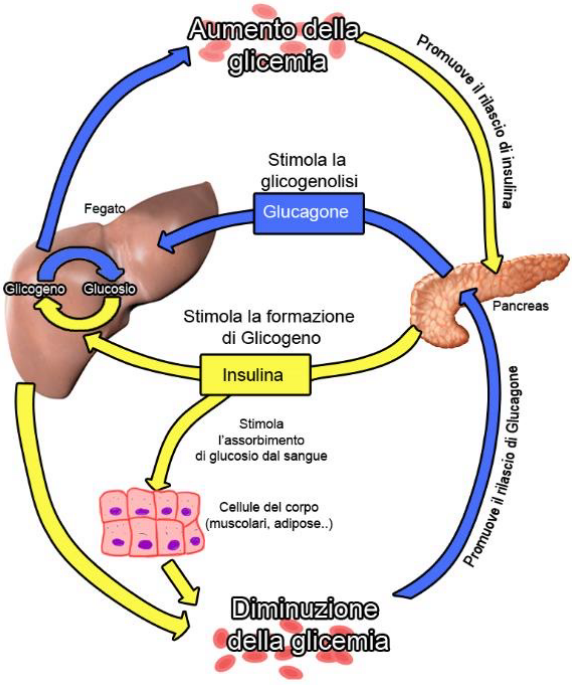
\includegraphics[width=.4\textwidth]{media/omeostasi.png}
    \vspace{-2.4cm}
\end{wrapfigure}
\phantom{}\\
\textbf{Omeostasi:}
\begin{itemize}
    \item La figura mostra come il corpo regola il livello di glucosio nel sangue attraverso due
        ormoni principali: l'insulina e il glucagone.
    \item Quando la glicemia aumenta, il pancreas rilascia insulina, che stimola l'assorbimento
        del glucosio nelle cellule e la formazione di glicogeno nel fegato.
    \item Quando la glicemia diminuisce, il pancreas rilascia glucagone, che stimola la
        glicogenolisi nel fegato, aumentando il livello di glucosio nel sangue.
    \item Questo meccanismo di feedback negativo mantiene la glicemia entro un intervallo
        normale.
\end{itemize}
\wrapfill

\subsection{Glicemia e regolazione del glucosio}
\begin{itemize}
    \item La glicemia è quella che regola il glucosio nel sangue;
    \item Quando c'è bisogno di tenere il glucosio all'interno delle cellule, canali adattivi
        si aggiungono e si tolgono.
\end{itemize}

\subsubsection{Iperglicemia}
\begin{itemize}
    \item L'insulina è il messaggero che dà l'informazione alle cellule che il livello di
        glicemia è alto, così da far attivare le cellule ad aprire i canali (Glut4);
    \item L'insulina viene creata dal pancreas;
    \item Le cellule del pancreas sono in grado di misurare la glicemia così da attivare la
        produzione di insulina.
\end{itemize}

\subsubsection{Ipoglicemia}
\begin{itemize}
    \item Il glucagone è il messaggero che dà l'informazione alle cellule che il livello di
        glicemia è basso;
    \item Anche il glucagone è creato dal pancreas.
\end{itemize}

\subsection{Reazioni tra enzimi e vie metaboliche}
\subsubsection{Gli enzimi}
Gli enzimi sono dei catalizzatori che servono garantire che avvengano determinate reazioni
chimiche.

\cfig{.6}{media/enzimi.png}

Ogni reazione ha il suo enzima dedicato.

\subsubsection{Reazioni non catalizzate}
Con l'assenza di un enzima che faciliti, la probabilità di urti efficaci che facciano avvenire
la reazione è estremamente passa.

\cfig{.75}{media/uncat.png}

\subsubsection{Reazioni catalizzate}
Con la presenza dell'enzima, le molecole si adagiano già nella posizione corretta così che
la collisione abbia una probabilità molto elevata che sia efficace e che la reazione chimica
avvenga.

\cfig{.75}{media/cat.png}

\subsubsection{Sito attivo}
L'enzima stimola i due reagenti a iniziare la transizione così che i due reagenti non sfruttino
il sito attivo solo come riparo.

\cfig{.75}{media/sito-attivo.png}

\subsubsection{Catalisi biologica}

\cfig{.75}{media/energy-reaction.png}

\subsubsection{Inibitori enzimatici}
Un inibitore enzimatico è una molecola in grado di instaurare un legame chimico con un enzima,
diminuendone così l'attività. Una molecola inibitrice, simile al reagente, può occupare il
sito attivo dell'enzima destinato al reagente, bloccando l'enzima e quindi la reazione chimica.
Gli inibitori sono prodotti quando è necessario ridurre il numero di reazioni chimiche,
ad esempio tramite feedback negativo o come farmaco.

Esistono due tipi di inibitori:
\begin{itemize}
    \item \textbf{Competitivo}: occupa il posto del reagente nel sito attivo.
    \item \textbf{Non competitivo}: deforma il sito attivo legandosi in un'altra posizione dell'enzima.
\end{itemize}

Entrambi i tipi di inibitori possono essere:
\begin{itemize}
    \item \textbf{Reversibili}: gli inibitori si legano momentaneamente all'enzima;
    \item \textbf{Irriversibili}: gli inibitori si legano covalentemente per sempre all'enzima.
\end{itemize}

\cfig{.8}{media/inibitori.png}

\subsubsection{Metabolismo}
Tutte le reazioni chimiche metaboliche sono suddivise in due gruppi:

\begin{center}
    \begin{tikzpicture}[
        level 1/.style = {sibling distance = 5cm},
        level 2/.style = {sibling distance = 3cm},
    ]
    \node {\Ovalbox{\large \textbf{Metabolismo}}}
        child {
            node {\ovalbox{Anabolismo}}
            child {
                node {\ovalbox{\makecell[l]{Produce molecole}}}
            }
        }
        child {
            node {\ovalbox{Catabolismo}}
            child {
                node {\ovalbox{\makecell[l]{Distrugge atomi, \\ piccole molecole}}}
            }
            child {
                node {\ovalbox{\makecell[l]{Libera energia \\ chimica}}}
            }
        };
    \end{tikzpicture}
\end{center}

\subsubsection{Anabolismo}
\begin{itemize}
    \item L'anabolismo è il processo metabolico che costruisce molecole complesse a partire da
        molecole più semplici;
    \item Richiede energia, che spesso viene fornita dall'ATP;
    \item Esempi di processi anabolici includono la sintesi proteica, la sintesi del DNA e la
        sintesi dei lipidi;
    \item Favorisce la crescita e la riparazione dei tessuti.
\end{itemize}

\subsubsection{Catabolismo}
\begin{itemize}
    \item Il catabolismo è il processo metabolico che scompone molecole complesse in molecole
        più semplici;
    \item Rilascia energia, che viene immagazzinata sotto forma di ATP;
    \item Esempi di processi catabolici includono la glicolisi, la respirazione cellulare e la
        degradazione degli acidi grassi;
    \item Fornisce l'energia necessaria per le attività cellulari.
\end{itemize}

\subsection{Respirazione cellulare}
Nella respirazione cellulare, il glucosio viene demolito fino alle molecole semplici di CO2 e
H2O, mentre viene consumato O2. L'energia liberata viene immagazzinata nelle molecole di ATP,
utilizzate dalla cellula per i vari processi metabolici. Parte dell'energia è dissipata come 
calore.

\subsubsection{Fasi della respirazione cellulare}
La respirazione cellulare include tre tappe principali:
\begin{enumerate}
    \item \textbf{Glicolisi}: avviene nel citoplasma delle cellule eucariotiche;
    \item \textbf{Ciclo di Krebs}: si svolge nella matrice mitocondriale;
    \item \textbf{Fosforilazione ossidativa}: avviene nella membrana interna dei mitocondri,
        comprende la catena di trasporto degli elettroni e la chemiosmosi.
\end{enumerate}

Nelle cellule procariotiche, le prime fasi avvengono nel citoplasma e la catena di trasporto
degli elettroni è incorporata nella membrana plasmatica.

\cfig{.8}{media/respirazione-cellulare.png}

\subsubsection{Mitocondrio}
\begin{itemize}
    \item Il mitocondrio è un organello nella cellula dove avviene parte della respirazione
        cellulare;
    \item È composto da due membrane, dividendo l'interno in una parte interna ed esterna.
\end{itemize}

\subsubsection{Creatina}
\begin{itemize}
    \item La creatina è una molecola che possiede un fosfato;
    \item Il suo scopo è aumentare la produzione di ADP.
\end{itemize}

\subsubsection{Glicolisi}
\begin{itemize}
    \item La glicolisi è una serie di reazioni chimiche che scompongono il glucosio in due
        molecole di piruvato:
        \chemscheme{C$_6$H$_{12}$O$_6$ + 6O$_2$ \arrow{->} 6CO$_2$ + 6H$_2$O + ATP}
    \item È un processo anaerobico che non richiede ossigeno.
    \item Durante la glicolisi, la cellula produce due molecole di NADH e due molecole di ATP,
        ricche di energia;
    \item I lieviti e alcuni batteri possono soddisfare il proprio fabbisogno energetico
        esclusivamente tramite la glicolisi;
    \item La maggior parte degli organismi richiede più energia, ottenuta dalle fasi
        successive della respirazione cellulare.
\end{itemize}

\subsubsection{Ciclo di Krebs}
\begin{itemize}
    \item Il piruvato, prodotto finale della glicolisi, subisce modificazioni chimiche prima
        di entrare nei mitocondri;
    \item Per ogni molecola di glucosio, la glicolisi produce due molecole di acetil-CoA e due
        molecole di NADH;
    \item Nel ciclo di Krebs entrano due molecole di acetil-CoA per ogni molecola di glucosio
        iniziale, producendo complessivamente 2 ATP, 6 NADH e 2 FADH$_2$;
    \item La principale funzione delle prime due tappe è alimentare la fosforilazione
        ossidativa tramite NADH e FADH$_2$.
\end{itemize}
\cfig{.6}{media/ciclo-di-krebs.png}

\subsubsection{Fosforilazione ossidativa}
\begin{itemize}
    \item La fosforilazione ossidativa avviene sulla membrana interna dei mitocondri;
    \item Comprende la catena di trasporto degli elettroni e la chemiosmosi;
    \item Il NADH e il FADH$_2$ cedono elettroni a un complesso di molecole che li trasportano
        fino all'ossigeno, formando H$_2$O;
    \item La chemiosmosi sfrutta l'energia liberata dai trasferimenti di elettroni per generare
        ATP;
    \item L'enzima ATP sintetasi utilizza l'energia potenziale per generare ATP, facendo
        passare gli ioni idrogeno attraverso un proprio canale.
\end{itemize}
\cfig{.9}{media/fosforilazione-ossidativa.png}

\subsubsection{Fermentazione}
La fermentazione è una via metabolica che permette agli organismi di ricavare energia in
assenza di ossigeno. Esistono due tipi di fermentazione:
\begin{enumerate}
\item \textbf{Fermentazione alcolica}
    \begin{itemize}
        \item Avviene nei lieviti e in alcuni batteri;
        \item Il piruvato viene trasformato in etanolo, rigenerando NAD+ e producendo CO$_2$.
    \end{itemize}
    \cfig{.8}{media/ferm-alcolica.png}
\item \textbf{Fermentazione lattica}
    \begin{itemize}
        \item Svolta da alcuni batteri e dagli esseri umani dopo uno sforzo muscolare;
        \item Il piruvato viene convertito in acido lattico, smaltito dal fegato con l'uso di
            ATP;
        \item In questo processo si rigenera il NAD+, necessario per la produzione di NADH
            durante la glicolisi.
    \end{itemize}
    \newpage
    \cfig{.8}{media/ferm-lattica.png}
\end{enumerate}

\subsubsection{Rigenerazione dell'ATP}
\cfig{.7}{media/atp.png}

\subsubsection{Lavoro cellulare}
\cfig{.7}{media/lavoro-cellulare.png}

\subsection{Fotosintesi}
La fotosintesi clorofilliana è un processo chimico mediante il quale le piante verdi e altri
organismi producono sostanze organiche, principalmente carboidrati. Utilizza come reagenti
principali l'anidride carbonica atmosferica e l'acqua metabolica, in presenza di luce solare.
Rientra tra i processi di anabolismo dei carboidrati, opposta ai processi di catabolismo.

La fotosintesi cattura l'energia luminosa del Sole e la utilizza per convertire acqua (H$_2$O) e
diossido di carbonio (CO$_2$) in zuccheri e ossigeno (O$_2$). Si svolge all'interno di organuli
specializzati chiamati cloroplasti.

La fotosintesi è un processo biochimico complesso suddiviso in due fasi principali:
\begin{enumerate}
    \item \textbf{Fase luminosa:}
    \begin{itemize}
        \item Richiede la presenza di luce;
        \item Avviene nelle membrane dei tilacoidi all'interno dei cloroplasti;
        \item L'energia luminosa viene convertita in energia chimica sotto forma di ATP e NADPH;
    \end{itemize}
    \item \textbf{Fase oscura (Ciclo di Calvin):}
    \begin{itemize}
        \item Non necessita di luce per svolgersi;
        \item Avviene nello stroma dei cloroplasti;
        \item Utilizza l'ATP e il NADPH prodotti nella fase luminosa per sintetizzare zuccheri
            a partire da CO$_2$.
    \end{itemize}
\end{enumerate}



\newpage
\section{Anatomia e fisiologia della cellula}
\subsection{Cellule}
\subsubsection{Cellule unicellulari}
Esistono due tipi di cellule unicellulari:
\begin{itemize}
    \item Cellule procariote, senza nucleo:\\
        Sono cellule prive di un nucleo ben definito e delimitato dalla membrana cellulare e
        da organelli;
    \item Cellule eucariote, con nucleo:\\
        Sono cellule che possiedono un nucleo circondato da una membrana, contenente DNA, e da
        organelli specializzati (es. mitocondri, reticolo plasmatico). 
\end{itemize}

\subsubsection{Cellule pluricellulari}
Le uniche cellule pluricellulari esistenti possono essere unicamente con un nucleo, dunque
solo cellule eucariote.

\subsubsection{Procariote}
\begin{itemize}
    \item Servono a ricavare energia dall glicolisi;
    \item Si muovono utilizzando i flagelli posti all'estremità della cellula.
\end{itemize}

\subsubsection{Eucariote}
\begin{itemize}
    \item Fanno la respirazione cellulare;
    \item La unicellulare si sposta singolarmente all'interno del corpo;
    \item La pluricellulare fa parte di un organismo;
    \item L'efficienza dello scambio cellulare è influenzata dal rapporto superficie-volume
        della cellula eucariote.
\end{itemize}

\cfig{.6}{media/cellule.png}

\newpage
\subsection{Cellule animali}
\subsubsection{Membrana plasmatica}
Membrana che separa tra l'interno e l'esterno della cellula e regola il passaggio di molecole.

\subsubsection{Nucleo}
Contiene il DNA e controlla l'attività cellulare. È circondato dall'\textbf{involucro nucleare},
il quale regola il flusso delle molecole.

\subsubsection{Sistema di membrane endocellulari}
È una rete di organelli che produce e distribuisce prodotti cellulari.

\subsubsection{Ribosomi}
Strutture responsabili della produzione delle proteine.

\subsubsection{Reticolo endoplasmatico}
Il RE è il principlae centro di produzione delle cellule, suddiviso in:
\begin{itemize}
    \item RE ruvido: ha ribosomi sulla superficie esterna e si occpua della sistetizzazione
        delle proteine;
    \item RE liscio: non ha ribosomi e si occupa della costruzione di lipidi.
\end{itemize}

\subsubsection{Apparato di Golgi}
Perfeziona, etichetta e invia le proteine alle loro destinazioni.

\subsubsection{Lisosoma}
Presenti unicamente nelle cellule animali.

Contengono enzimi digestivi che demoliscono tramite idrolisi macromolecole che vengono poi
riciclate.

\subsubsection{Mitocondrio}
Organello principale per la produzione di energia attraverso la respirazione cellulare.
Trasforma gli zuccheri in ATP.

\subsubsection{Citoscheletro}
È una struttura di sostegno che dà forma alla cellula e fornisce punti di attacco per gli
altri organelli.

\subsection{Cellule vegetali}
\subsubsection{Parete cellulare}
Strato rigido esterno che protegge la cellula, composto da cellulosa, altri polisaccaridi e
proteine.

\subsubsection{Vacuolo centrale}
Organello che serve a regolare lo stoccaggio d'acqua nella cellula e a demolire i prodotti di
scarto.

\subsubsection{Cloroplasto}
Organello in cui si svolgono le reazioni della fotosintesi. L'energia solare viene trasformata
in zuccheri.

\newpage
\subsection{Sintetizzazione delle proteine}
\cfig{.8}{media/sint-proteine}

\subsubsection{Nel citoplasma}
\begin{itemize}
    \item Gli amminoacidi entrano per diffusione passiva;
    \item L'RNA dà l'informazione al ribosoma;
    \item Il ribosoma legge l'informazione e mette in fila ordinata gli amminoacidi;
    \item Dopo aver sintetizzato la proteina, il ribosoma la spedisce fuori dal citoplasma
        (oppure rimane nel citoplasma se esso è la sua destinazione);
    \item La proteina viene spedita nel ritocolo endoplasmatico ruvido, con direzione il punto
        vescicolare, unendosi con le altre proteine;
    \item La vescicola si stacca e si fonde con la membrana per creare nuovi fosfolipidi che
        serviranno per la rigenerazione del reticolo endoplasmatico.
\end{itemize}

\cfig{.6}{media/sint-citoplasma.png}

\newpage
\subsubsection{Gli organi cellulari in breve}
\vspace*{0.5cm}
\begin{tabular}{| m{.5cm} |}
    \hline \cellcolor{darkgreen!50} \phantom{} \\ \hline
\end{tabular} Cellule unicamente vegetali

\begin{tabular}{| m{.5cm} |}
    \hline \cellcolor{blue!50} \phantom{} \\ \hline
\end{tabular} Cellule unicamente animali

\vspace*{.5cm}
\begin{table}[h!]
    \centering
    \begin{tabular}{| m{3cm} | m{3cm} | m{3cm} | m{3cm} |}
    \hline
    \textbf{Controllo dell’informazione genetica} & \textbf{Produzione di energia} & \textbf{Costruzione, distribuzione e degradazione} & \textbf{Supporto fisico, movimento e comunicazione tra le cellule} \\ \hline
    Nucleo  & \textcolor{darkgreen}{Cloroplasti}  & \textcolor{darkgreen}{Vacuoli} & \textcolor{darkgreen}{Parete cellulare} \\ \hline
    Ribosomi & Mitocondri & \textcolor{blue}{Lisosoma} & Flagelli \\ \hline
     &  & RE ruvido & Citoscheletro \\ \hline
     &  & RE liscio & Giunzioni cellulari \\ \hline
     &  & Apparato di Golgi & Membr. plasmatica \\ \hline
     &  & Ribosomi & \begin{tabular}{l} \hspace*{-.3cm} Matrice \\ \hspace*{-.3cm} extracellulare \end{tabular} \\ \hline
     &  & Perossisomi &  \\ \hline
    \end{tabular}
\end{table}

\subsection{La diffusione attraverso la membrana}
\subsubsection{Gradiente di concentrazione}
Lo spostamento della materia attraverso una membrana permeabile avviene tramite diffusione
semplice per gradiente di concentrazione. Per contrastare la diffusione, la cellula deve
investire energia (trasporto contro gradiente)

\cfig{.7}{media/gradiente.png}
\vspace*{0.5cm}

\setlength{\intextsep}{0pt}%
\begin{wrapfigure}{l}{0.4\textwidth}
    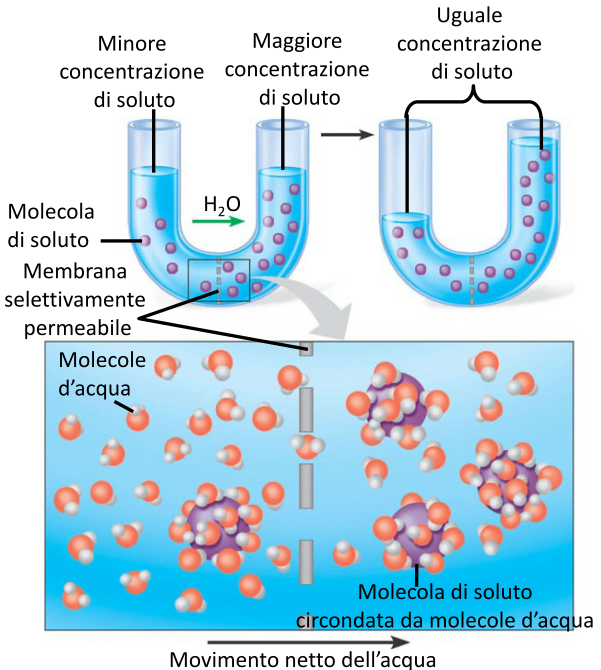
\includegraphics[width=.4\textwidth]{media/osmosi.png}
    \vspace{-2.4cm}
\end{wrapfigure}
\phantom{}

\subsubsection{Osmosi}
Quando la membrana è semipermeabile, il soluto non può spostarsi, di conseguenza
\underline{si sposta il solvente}. L'osmosi avviene solo quando la membrana è semipermeabile
e consiste nel movimento passivo dell'acqua da dove la soluzione è meno concentrata a dove è
più concentrata.

\subsubsection{Osmoregolazione}
Intervento attivo che fanno le cellule per mantenere costante il bilancio idrico delle cellule
per evitare le conseguenze dell'autoregolazione dell'acqua.
\wrapfill

\subsection{Equilibrio idrico}
\subsubsection{Soluzione isotonica (E=I)}
\begin{itemize}
    \item La concentrazione di acqua è uguale sia all'interno sia all'esterno della cellula,
        figura (\textit{A,D});
    \item La cellula animale si trova a condizione normale;
    \item La cellula vegetale perde di tugore poiché abituata all'assorbimento di tanta acqua.
\end{itemize}

\subsubsection{Soluzione ipotonica (E$>$I)}
\begin{itemize}
    \item La concentrazione all'interno della cellula è minore di quella esterna,
        figura \textit{(B,E)};
    \item L'acqua tende, per gradiente di concentrazione, ad entrare nella cellula;
    \item La cellula animale si gonfia poiché il flusso dell'acqua va dall'esterno all'interno
        ed esplode;
    \item La cellula vegetale ha bisogno dell'assorbimento dell'acqua e dunque sarà turgida.
\end{itemize}

\subsubsection{Soluzione ipertonica (E$<$I)}
\begin{itemize}
    \item La concentrazione all'interno della cellula è maggiore di quella esterna,
        figura \textit{(C,F)};
    \item L'acqua tende, per gradiente di concentrazione, ad uscire dalla cellula:
    \item La cellula animale raggrinzisce;
    \item La cellula vegetale raggrinzisce.
\end{itemize}

\cfig{.9}{media/equilibrio-idrico.png}

\newpage
\section{La nutrizione}
\subsection{Anatomia digestiva}
\cfig{1}{media/anatomia-digestiva.png}

\subsubsection{Stomaco}
\setlength{\intextsep}{0pt}%
\begin{wrapfigure}{l}{0.6\textwidth}
    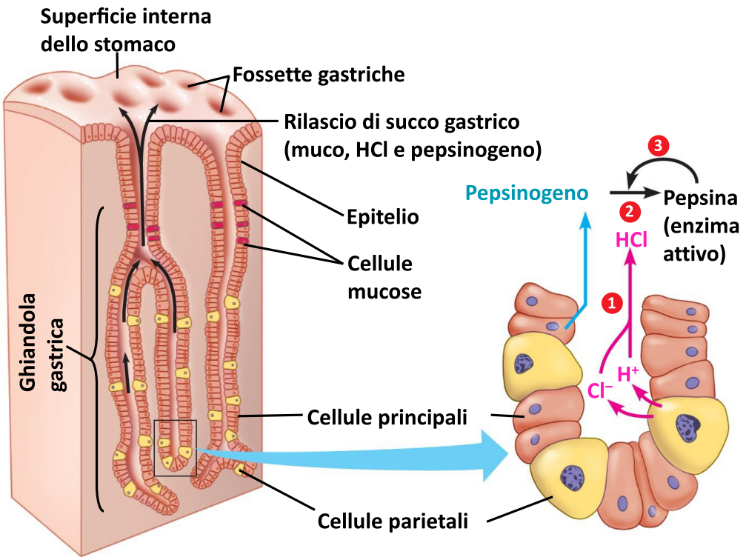
\includegraphics[width=.6\textwidth]{media/stomaco.png}
    \vspace{-2.4cm}
\end{wrapfigure}
\phantom{}

\textbf{Cellule dello stomaco:}
\begin{itemize}
    \item Cellule parietali: rilasciano HCl;
    \item Cellule principali: rilasciano il pepsinogeno (che diventa pepsina con il rilevamento
        di HCl);
    \item Cellule G: rilasciano l'ormone della gastrina, il quale regola le ghiandole gastriche;
    \item Cellule mucose: rilasciano mucina.
\end{itemize}
\wrapfill

\newpage
\subsection{Assorbimento delle sostanze nutritive}
\subsubsection{Intestino tenue}
\setlength{\intextsep}{0pt}%
\begin{wrapfigure}{l}{0.25\textwidth}
    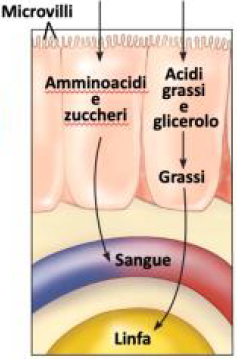
\includegraphics[width=.25\textwidth]{media/intestino.png}
    \vspace{-2.4cm}
\end{wrapfigure}
\phantom{}\\
L'intestino tenue è formato da villi posizionati sulla superficie interna. A loro volta, i
villi sono formati da microvilli, i quali servono ad aumentare la superficie attiva per
l'assorbimento delle sostanze.

Nell'intestino vengono assorbiti
\begin{itemize}
    \item Monosaccaridi;
    \item Amminoacidi;
    \item Acidi grassi e glicerolo;
    \item Nucleotidi;
    \item Vitamine;
    \item Acqua;
    \item Sali minerali.
\end{itemize}
\wrapfill

\subsubsection{Idrolisi enzimatica}
Tutti i nutrenti sopracitati vengono scomposti tramite idrolisi, successivamente assorbiti
dai vasi sanguigni e trasferiti verso il fegato.

\subsubsection{Lipidi}
I lipidi idrofobi e alcune vitamine non vengono assorbiti nel sangue, ma oltrepassano il vaso
sanguigno per venire assorbiti direttamente dalla linfa (sistema linfatico).

\cfig{.8}{media/digestione.png}

\newpage
\subsection{Dosi da assumere giornaliere}
\begin{itemize}
    \item Tasso metabolico: tasso di consumo energetico dell'organismo che serve a far
        sopravvivere gli organismi durante il sonno o un eventuale coma;
    \item Metabolismo basale: numero di kcal necessarie per alimentare in un determinato
        momento i processi vitali di un animale durante il riposo (respirazione, battito
        cardiaco);
    \item Consumo energetico aggiuntivo.
\end{itemize}

Il totale di queste tre suddivisioni è di circa:
\begin{itemize}
    \item Uomini: 1600-1800 kcal/giorno;
    \item Donne: 1300-1500 kcal/giorno.
\end{itemize}

\newpage
\section{Il sistema cardiocircolatorio}
\subsection{Il sistema cardiocircolatorio umano}
Il sistema cardiocircolatorio è un sistema chiuso costituito da organismi pluricellulari,
vasi sanguigni, sangue e flussi di materia e nutrienti.

\subsubsection{La circolazione sanguigna}
{\color{red}{\textbf{Questo vale SOLO per il sistema cardiocircolatorio!!}}}
\begin{itemize}
    \item Porta nutrienti (es. H$_2$O);
    \item Porta via scarti (es. CO$_2$);
    \item Regola alcuni parametri corporei.
\end{itemize}

\subsubsection{Funzioni del sangue}
\begin{itemize}
    \item Trasporto dei gas:
        \begin{itemize}
            \item O$_2$: Polmoni\ \textrightarrow\ Sangue\ \textrightarrow\ Cellule (trasporto
                attivo, gradiente di concentrazione);
            \item CO$_2$: Cellule\ \textrightarrow\ Sangue\ \textrightarrow\ Polmoni;
        \end{itemize}
    \item Metabolismo:
        \begin{itemize}
            \item Metaboliti assunti (nutrienti);
            \item Metaboliti scartati (scarti);
        \end{itemize}
    \item Nel fegato:
        \begin{itemize}
            \item Detossificazione delle sostanze (modifica dei metaboliti);
        \end{itemize}
    \item Nei reni:
        \begin{itemize}
            \item Espulsione dei metaboliti scartati;
        \end{itemize}
    \item Nei muscoli:
        \begin{itemize}
            \item Scambio tra scarti e nutrienti tra capillari e muscoli;
        \end{itemize}
    \item Trasporto di ormoni:
        \begin{itemize}
            \item Le ghiandole endocrine mandano messaggi sfruttando il percorso del sangue;
        \end{itemize}
    \item Omeostasi:
        \begin{itemize}
            \item Termoregolazione: alzare e/o abbassare la temperatura degli organi;
            \item Water balance: cambia le concentrazioni dei soluti nel sangue per mantenere
                l'equilibrio idrico;
            \item Acidità: vengono lanciate sostanze acide o basiche che mantengono il pH
                bilanciato;
        \end{itemize}
    \item Difesa:
        \begin{itemize}
            \item Cellule: trasporto di globuli bianchi che distruggono gli organismi patogeni;
            \item Proteine: trasporto di anticorpi per la difesa da agenti patogeni;
            \item Coagulati: trasporto di piastrine (pezzi di cellule) e fibrine (pezzi di
                proteine).
        \end{itemize}
\end{itemize}

\newpage
\subsubsection{Composizione del sangue}
\vspace*{0.5cm}
\begin{table}[ht!]
    \centering
    \arrayrulecolor{black}
    \setlength{\extrarowheight}{4pt}
    \renewcommand{\arraystretch}{1.5}
    \begin{tabular}{|p{4cm}|p{5cm}|p{4cm}|}
    \hline
    \multicolumn{3}{|c|}{\textbf{\textcolor{red}{Elementi cellulari (45\%)}}} \\ \hline
    \textbf{Tipi di cellule} & \textbf{Funzioni} & \textbf{Info} \\ \hline
    Eritrociti (globuli rossi) & Trasporto di O$_2$ e, in parte, di CO$_2$ & No nucleo; \newline Più superficie possibile \\ \hline
    Leucociti (globuli bianchi) & Difesa ed immunità & - \\ \hline
    Piastrine & Coagulazione del sangue & Frammenti di cellule \\ \hline
    \end{tabular}
\end{table}
\vspace*{1cm}
\begin{table}[h!]
    \centering
    \arrayrulecolor{black}
    \setlength{\extrarowheight}{4pt}
    \renewcommand{\arraystretch}{1.5}
    \begin{tabular}{|p{5cm}|p{8.5cm}|}
    \hline
    \multicolumn{2}{|c|}{\textbf{\textcolor{red}{Plasma (55\%)}}} \\ \hline
    \textbf{Componenti} & \textbf{Funzioni principali} \\ \hline
    Acqua & Solvente per diluire le altre sostanze \\ \hline
    \begin{tabular}[c]{@{}l@{}}Ioni organici: \\ Sodio; Potassio; Calcio; \\ Magnesio; Cloruro; Bicarbonato\end{tabular} & \begin{tabular}[c]{@{}l@{}}Azione tampone (pH), equilibrio osmotico, equilibrio \\ ionico del flusso interstiziale, trasmissione di impulsi \\ nervosi.\end{tabular} \\ \hline
    \begin{tabular}[c]{@{}l@{}}Proteine plasmatiche: \\ 1) Albumina; \\ 2) Fibrinogeno; \\ 3) Immunoglobuline.\end{tabular} & \begin{tabular}[c]{@{}l@{}}1) Equilibrio osmotico e azione tampone (pH) \\ \hspace*{0.4cm}(cambio concentrazioni); \\ 2) Coagulazione (fibrina inattiva); \\ 3) Immunità (anticorpi).\end{tabular} \\ \hline
    \multicolumn{2}{|p{8.5cm}|}{\begin{tabular}[c]{@{}l@{}}Sostanze trasportate dal sangue: \\ Sostanze nutritive; \\ Prodotti di rifiuto del metabolismo; \\ Gas respiratori (O$_2$ e CO$_2$); \\ Ormoni.\end{tabular}} \\ \hline
    \end{tabular}
\end{table}

\subsubsection{Il sistema umano}
\begin{itemize}
    \item Sangue: fluido circolante (plasma + elementi cellulari);
    \item Sistema di vasi:
        \begin{itemize}
            \item Arterie: portano via il sangue dall'organo;
            \item Arteriole;
            \item Vene: roportano indietro il sangue verso l'organo;
            \item Venule;
            \item Capillari;
        \end{itemize}
    \item Cuore: pompa, motore che permette la circolazione del sangue.
\end{itemize}

\subsection{Il cuore}
\subsubsection{Biologia del cuore}
\begin{itemize}
    \item 4 cavità cardiache: il cuore umano è più performante di altre specie animali;
    \item Circolazione sanguigna:
        \begin{itemize}
            \item Circolazione sistematica: il sangue va in tutto il corpo;
            \item Circolazione polmonare: il sangue va verso e torna dai polmoni;
        \end{itemize}
    \item Il cuore soddisfa elevate necessità metaboliche:
        \begin{itemize}
            \item Mantiene sempre il sangue in temperatura: costante apporto di ATP;
            \item Trasporta in brevissimo tempo tanti nutrienti e ossigeno alle cellule.
        \end{itemize}
\end{itemize}

\subsubsection{Evoluzione del sistema cardiocircolatorio nei vertebrati}
\cfig{.8}{media/evoluzione-cuore.png}

\subsubsection{Anatomia del cuore umano}
\cfig{.9}{media/anatomia-cuore.png}

\begin{itemize}
    \item Valvole semilunari: si aprono con la contrazione del cuore (normalmente chiuse);
    \item Valvole ventricolari: si aprono con la depressione del cuore (normalmente aperte).
\end{itemize}

\subsubsection{Schema circolatorio}

\cfig{.6}{media/schema-cuore.png}

\subsubsection{Direzione di scorrimento dei flussi}
\cfig{.5}{media/circ-cuore.png}

\newpage
\subsubsection{Circolazione sanguigna}
\cfig{1}{media/circ-sanguigna.png}

\subsection{Il ciclo cardiaco}
\subsubsection{Le fasi del ciclo cardiaco}
\setlength{\intextsep}{0pt}%
\begin{wrapfigure}{l}{.5\textwidth}
    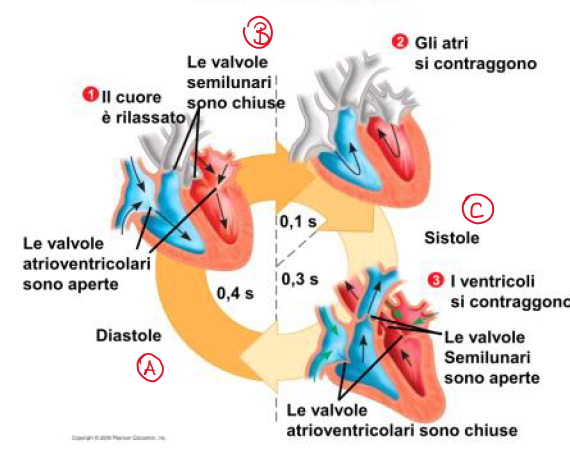
\includegraphics[width=.5\textwidth]{media/ciclo-cardiaco.png}
    \vspace{-2.4cm}
\end{wrapfigure}
\phantom{}\\
\begin{enumerate}[label=\Alph*)]
    \item Diastole;
    \item Sistole arteriale;
    \item Sistole ventricolare.
\end{enumerate}
\wrapfill

\subsubsection{Diastole}
La diastole è il rilassamento del muscolo cardiaco:
\begin{itemize}
    \item Le valvole atrioventricolari sono tutte aperte e il sangue ci fluisce attraverso
        (0.4 s).
\end{itemize}

\subsubsection{Sistole atriale}
Gli atri vengono strizzati per far fluire tutto il sangue:
\begin{itemize}
    \item Vengono riempiti al massimo i ventricoli;
    \item Le valvole semilunatiche sono ancora chiuse.
\end{itemize}

\subsubsection{Sistole ventricolare}
I ventricoli vengono strizzati per far partire il flusso sanguigno ad alta pressione nelle
arterie:
\begin{itemize}
    \item Le valvole ventricolari sono completamente chiuse;
    \item Le valvole semilunatiche si aprono con la pressione del fluido.
\end{itemize}

\subsection{Segnali elettrici del cuore}
\subsubsection{Nodo senoatriale (pacemaker)}
\setlength{\intextsep}{0pt}%
\begin{wrapfigure}{l}{.25\textwidth}
    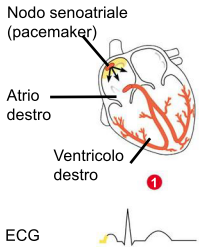
\includegraphics[width=.25\textwidth]{media/pacemaker.png}
    \vspace{-2cm}
\end{wrapfigure}
\phantom{}\\
\begin{itemize}
    \item La regolazione del ritmo cardiaco avviene grazie a zone specializzate del tessuto
        muscolare del cuore;
    \item Il nodo senoatrale genera dapprima impulsi elettrici e poi mantiene il ritmo del
        pompaggio regolare.
\end{itemize}
\wrapfill

\subsubsection{Nodo atrioventricolare (AV)}
\setlength{\intextsep}{0pt}%
\begin{wrapfigure}{l}{.25\textwidth}
    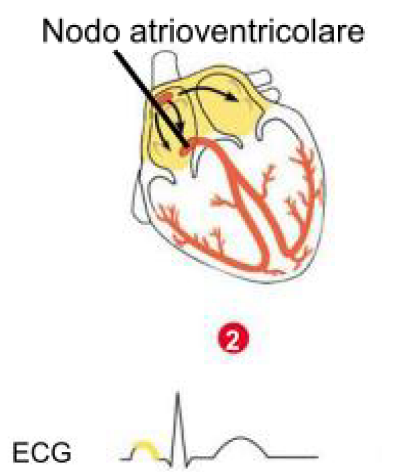
\includegraphics[width=.25\textwidth]{media/nodo-av.png}
    \vspace{-2cm}
\end{wrapfigure}
\phantom{}\\
\begin{itemize}
    \item I segnali dal nodo senoatrale si propagano attraverso gli atri:
        \begin{itemize}
            \item Contrazione simultanea dei due atri;
        \end{itemize}
    \item Il segnale arriva al nodo atrioventricolare (AV)
        \begin{itemize}
            \item Trasmissione di impulsi elettrici;
            \item Rallenta la frequenza del pacemaker per far contrarre i ventricoli qualche
                secondo prima degli altri.
        \end{itemize}
\end{itemize}
\wrapfill

\subsubsection{Fibre muscolari specializzate (regolazione del ritmo cardiaco)}
\setlength{\intextsep}{0pt}%
\begin{wrapfigure}{l}{.25\textwidth}
    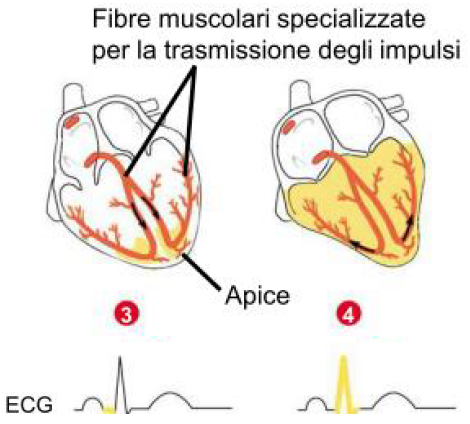
\includegraphics[width=.25\textwidth]{media/fibre-muscolari.png}
    \vspace{-2cm}
\end{wrapfigure}
\phantom{}\\
\begin{itemize}
    \item I segnali dal nodo senoatrale si propagano attraverso gli atri:
        \begin{itemize}
            \item Contrazione simultanea dei due atri;
        \end{itemize}
    \item Il segnale arriva al nodo atrioventricolare (AV)
        \begin{itemize}
            \item Trasmissione di impulsi elettrici;
            \item Rallenta la frequenza del pacemaker per far contrarre i ventricoli qualche
                secondo prima degli altri.
        \end{itemize}
\end{itemize}
\wrapfill

\subsubsection{Iperpolarizzazione}
\cfig{1}{media/iperpolarizzazione.png}

\newpage
\subsubsection{Circolazione coronaria}
Le arterie coronarie alimentano il cuore.
\cfig{.6}{media/coronaria.png}

\subsection{Malattie dell'apparato cardiocircolatorio}
\subsubsection{Aterosclerosi}
L'aterosclerosi cosiste nella formazione di placche (ateromi) all'interno delle pareti delle
arterie, rendendo molto difficoltoso lo scorrimento del sangue.

Conseguenze:
\begin{itemize}
    \item Attacco cardiaco (infarto del miocardio): causato dall'ostruzione di una o più
        arterie coronarie. Il flusso di sangue si blocca e un gruppo di cellule del cuore
        muore.
    \item Ictus celebrale: si verifica quando viene interrotto l'apporto di sangue in un'area
        del cervello.
\end{itemize}

\subsection{La pressione sanguigna}
\cfig{1}{media/pressione.png}

\newpage
\subsubsection{Pressione sistolica}
La pressione al momento in cui il ventricolo viene contratto (120mmHg).

\cfig{.4}{media/sistolica.png}

\subsubsection{Pressione diastolica}
La pressione al momento in cui il cuore si rilassa (70/80mmHg).

\cfig{.4}{media/diastolica.png}

\subsubsection{Funzionamento dello sfigmomanometro}
\begin{enumerate}
    \item Il bracciale si gonfia di molto così da impedire il flusso sanguigno di circolare;
    \item Si sgonfia regolarmente finché il flusso non riparte;
    \item Quando riparte il fluido, l'apparecchio annota la pressione massima (sistolica);
    \item Continua a sgonfiarsi regolarmente finché il bracciale non percepisce più il flusso
        sanguigno sulla parete dell'arteria, annotando la pressione minima (diastolica).
\end{enumerate}

\cfig{.9}{media/sfigmomanometro.png}

\newpage
\subsubsection{La velocità di scorrimento del sangue}

\cfig{1}{media/velocita-sangue.png}

\begin{itemize}
    \item Il sangue che scorre nella vena significa che sta tornando all’organo principale;
    \item Per far sì che il sangue arrivi fino al cuore, i muscoli si contraggono così da
        applicare una pressione sulla vena la quale spinge il flusso verso avanti;
    \item Per evitare che il flusso torni indietro, ogni tot ci sono delle valvole di non
        ritorno che sono apribili solo dal verso del flusso;
    \item Con il fluido che procede nel verso opposto le valvole non si riescono ad aprire.
\end{itemize}

\newpage
\section{Il sistema respiratorio}





















\end{document}